% !TeX root = ./forallxdo.tex
% Chapter on modal logic. Author of English original: Rob Trueman, http://www.rtrueman.com/

\part{Modale Logik}
\label{ch.ML}
\addtocontents{toc}{\protect\mbox{}\protect\hrulefill\par}

\chapter{Einführung in die modale Logik}
\label{Intro}

Die modale Logik (ML) ist die Logik der \emph{Modalitäten}, der Weisen, auf die ein Satz wahr sein kann. \emph{Notwendigkeit} und \emph{Möglichkeit} sind zwei solche Modalitäten: ein Satz kann wahr sein, aber er kann auch notwendigerweise wahr sein (wahr, egal wie die Welt auch beschaffen sein mag). Logische Wahrheiten sind z.B.\@ nicht nur zufälligerweise wahr. Sie sind notwendigerweise wahr. Ein Satz kann möglicherweise wahr sein, selbst, wenn er nicht tatsächlich wahr ist. Wir benutzen $\ebox$, um die Notwendigkeit auszudrücken und $\ediamond$, um die Möglichkeit auszudrücken. Sie können also $\ebox \metav{A}$ als \emph{Es ist notwendigerweise der Fall, dass} $\metav{A}$ und $\ediamond \metav{A}$ als \emph{Es ist möglicherweise der Fall, dass} $\metav{A}$ verstehen.

Es gibt viele verschiedene Arten von Notwendigkeiten. Es ist \emph{menschlich} unmöglich für mich, 100 Km/h schnell zu laufen. Angesichts der Art von Tier, das der Mensch ist, kann das kein Mensch tun. Aber dennoch ist es für mich \emph{physikalisch} nicht unmöglich, so schnell zu laufen. Wir haben noch nicht die Technologie dafür, aber es ist sicher physikalisch möglich, meine menschlichen Beine gegen Roboterbeine auszutauschen, mithilfe derer ich dann 100 Km/h schnell laufen kann. Im Gegensatz dazu ist es für mich physikalisch unmöglich, schneller als mit Lichtgeschwindigkeit zu laufen. Die Gesetze der Physik verbieten es jedem Objekt, auf diese Geschwindigkeit zu beschleunigen. Aber rein \emph{logisch} gesehen ist selbst das nicht unmöglich. Es ist kein Widerspruch, sich vorzustellen, dass die Gesetze der Physik anders sind und sie es Dingen erlauben, sich schneller als das Licht zu bewegen.

Mit welcher Art von Modalität befasst sich ML? \emph{Mit allen!} ML ist ein sehr flexibles Werkzeug. Wir beginnen mit einigen grundlegenden Regeln, die für $\ebox$ und $\ediamond$ gelten, und fügen dann weitere Regeln hinzu, um verschiedene Modalitäten zu repräsentieren. Tatsächlich ist ML so flexibel, dass wir $\ebox$ und $\ediamond$ nicht einmal so verstehen müssen, dass sie \emph{Notwendigkeit} und \emph{Möglichkeit} ausdrücken. Wir könnten stattdessen $\ebox$ als Ausdruck der \emph{Beweisbarkeit} lesen, so dass wir $\ebox\metav{A}$ als \emph{es ist beweisbar, dass} $\metav{A}$ und $\ediamond\metav{A}$ als \emph{es ist nicht widerlegbar, dass} $\metav{A}$ verstehen. In ähnlicher Weise können wir $\ebox\metav{A}$ so interpretieren, dass $S$ \emph{wei{\ss}, dass $\metav{A}$} oder $S$ \emph{glaubt, dass $\metav{A}$} bedeutet. Oder wir können $\ebox$ als Ausdruck einer \emph{moralischen Verpflichtung} lesen, so dass $\ebox \metav{A}$ bedeutet, dass $\metav{A}$ moralisch verpflichtend ist, und $\ediamond \metav{A}$, dass $\metav{A}$ moralisch zulässig ist. Alles, was wir tun müssen, um diese verschiedenen Interpretationen zu erhalten, ist, die richtigen Regeln für diese unterschiedlichen Lesarten von $\ebox$ und $\ediamond$ auszuarbeiten.

Ein modaler Satz ist einer, der modale Operatoren wie $\ebox$ und $\ediamond$ beinhaltet. Je nach Interpretation, die wir $\ebox$ und $\ediamond$ zuweisen, werden unterschiedliche modale Sätze beweisbar oder gültig sein. Zum Beispiel: $\ebox \metav{A} \eif \metav{A}$ könnte sagen, dass `wenn $\metav{A}$ notwendig ist, dann ist es wahr,' solange wir $\ebox$ als Notwendigkeit interpretieren. Oder es könnte besagen, dass `wenn $S$ wei{\ss}, dass $\metav{A}$, dann ist es wahr,' solange $\ebox$ das Wissen ausdrückt. Unter diesen beiden Interpretationen ist $\ebox\metav{A} \eif \metav{A}$ gültig: Alle Sätze die notwendigerweise wahr sind, sind tatsächlich wahr. Und wenn jemand wei{\ss}, dass $\metav{A}$, dann ist $\metav{A}$ wahr (denn man kann nicht wissen, was falsch ist). Wenn jedoch $\ebox$ als `es wird geglaubt, dass' oder `es sollte der Fall sein, dass' interpretiert wird, dann ist $\ebox\metav{A} \eif \metav{A}$ nicht gültig: Wir können falschen Behauptungen glauben schenken. Und nicht jeder Satz, der wahr sein sollte, ist tatsächlich wahr, z.B.\@: `Niemand begeht Morde'. Dieser Satz \emph{sollte} wahr sein, ist es aber leider nicht. 

Wir werden verschiedene Systeme der ML in Betracht ziehen. Sie unterscheiden sich in ihren Herleitungsregeln und in der Semantik, die wir verwenden, um unsere logischen Begriffe zu definieren. Die verschiedenen Systeme, die wir betrachten werden, hei{\ss}en \mlK, \mlT, \mlSfour{} und \mlSfive. \mlK{} ist das Basissystem; alles, was in \mlK{} gültig oder beweisbar ist, ist auch in den anderen beweisbar. Aber es gibt einige Dinge, die in \mlK{} nicht beweisbar sind, wie zum Beispiel der Satz $\ebox A \eif A$ für einen beliebigen Satzbuchstaben~$A$. Daher ist \mlK{} keine angemessene modale Logik für Notwendigkeit und Möglichkeit; denn hier sollte $\ebox\metav{A} \eif \metav{A}$ beweisbar sein. System \mlT{} stellt sich hierfür als besser geeignet heraus. Denn in diesem System ist $\ebox\metav{A} \eif \metav{A}$ beweisbar. \mlT{} ist also bei der Behandlung von Notwendigkeit und Möglichkeit angemessener, aber weniger angemessen, wenn es wir uns mit Glauben oder der moralischen Verpflichtung beschäftigen wollen, da dann $\ebox\metav{A} \eif \metav{A}$ \emph{nicht} (immer) beweisbar sein sollte. Das vielleicht beste System der ML für Notwendigkeit und Möglichkeit, auf jeden Fall das am weitesten verbreitete, ist das stärkste der von uns betrachteten Systeme, \mlSfive.

\section{Die Sprache der modalen Logik}
\label{TFLtoML}

Um die modale Logik anzuwenden, müssen wir zwei Dinge tun. Erstens wollen wir lernen, wie wir Dinge in der ML beweisen können. Zweitens wollen wir sehen, wie man Interpretationen für die ML konstruiert. Aber bevor wir diese beiden Dinge tun können, müssen wir erklären, wie man Sätze in der ML konstruiert.

Die Sprache der ML ist eine Erweiterung der WFL. Wir könnten auch auf Basis der LEO beginnen, dann würden wir die Quantifizierte Modale Logik (QML) erhalten. QML ist viel ausdrucksstärker als die ML, aber sie ist auch viel, viel komplizierter. Wir werden die Dinge also einfach halten und mit WFL beginnen.

Genau wie die WFL beginnt die ML mit einem unendlichen Vorrat an \emph{Basiselementen}. Diese werden als Gro{\ss}buchstaben geschrieben, mit oder ohne tiefgestellten Nummern: $A$, $B$, $\dots$ $A_1$, $B_1$, $\dots$ Wir nehmen dann alle Regeln, wie man Sätze aus WFL bildet, und fügen zwei weitere für $\ebox$ und $\ediamond$ hinzu:
\begin{itemize}
	\item[(1)]Jedes Basiselement der ML ist ein Satz der ML.
	\item[(2)]Wenn $\metav{A}$ ein Satz der modalen Logik ist, dann ist $\enot\metav{A}$ ein Satz der ML.
	\item[(3)]Wenn $\metav{A}$ und $\metav{B}$ Sätze der ML sind, dann ist $(\metav{A}\eand\metav{B})$ ein Satz der ML.
	\item[(4)]Wenn $\metav{A}$ und $\metav{B}$ Sätze der ML sind, dann ist $(\metav{A}\eor\metav{B})$ ein Satz der ML.
	\item[(5)]Wenn $\metav{A}$ und $\metav{B}$ Sätze der ML sind, dann ist $(\metav{A}\eif\metav{B})$ ein Satz der ML.
	\item[(6)]Wenn $\metav{A}$ und $\metav{B}$ Sätze der ML sind, dann ist $(\metav{A}\eiff\metav{B})$ ein Satz der ML.
	\item[(7)]Wenn $\metav{A}$ ein Satz der ML ist, dann ist $\ebox\metav{A}$ ein Satz der ML.
	\item[(8)]Wenn $\metav{A}$ ein Satz der ML ist, dann ist $\ediamond\metav{A}$ ein Satz der ML.
	\item[(9)]Nichts anderes ist ein Satz der ML.
\end{itemize}
Hier sind einige Beispiele:
\begin{itemize}
	\item[]$A,\;P\eor Q,\;\ebox A,\;C\eor \ebox D,\;\ebox\ebox (A\eif R),\;\ebox\ediamond (S\eand (Z\eiff (\ebox W \eor \ediamond Q)))$
\end{itemize}

\chapter{Natürliche Herleitung für die ML}
\label{Proof}

Jetzt, da wir wissen, wie wir in der ML Sätze bilden, können wir uns ansehen, wie wir in der ML Dinge herleiten können. Wir werden $\proves$ verwenden, um Beweisbarkeit auszudrücken. So bedeutet $\metav{A}_1,\metav{A}_2, \dots \metav{A}_n \proves \metav{C}$, dass $\metav{C}$ von $\metav{A}_1,\metav{A}_2, \dots \metav{A}_n$ aus hergeleitet werden kann. Wir werden uns jedoch mit einer Reihe verschiedener Systeme der ML befassen. Daher wird es nützlich sein, ein Subskript hinzuzufügen, das angibt, mit welchem System wir arbeiten. Wenn wir also zum Beispiel sagen wollen, dass wir $\metav{C}$ von $\metav{A}_1,\metav{A}_2, \dots \metav{A}_n$ \emph{in System}~\mlK{} aus herleiten können, dann schreiben wir: $\metav{A}_1,\metav{A}_2, \dots \metav{A}_n \proves_\mlK \metav{C}$.

\section{System \mlK}
\label{K}

Wir beginnen mit einem besonders einfachen System namens \mlK, benannt nach dem Philosophen und Logiker Saul Kripke. \mlK{} umfasst alle natürlichen Herleitungsregeln der WFL, einschlie{\ss}lich der abgeleiteten Regeln sowie der Grundregeln. \mlK{} fügt dann eine besondere Art von Unterbeweis hinzu, sowie zwei neue Grundregeln für $\ebox$.

Die spezielle Art des Unterbeweises sieht gewöhnlich aus; au{\ss}er, dass er statt eines Satzes ein $\ebox$ in seiner Annahmezeile hat. Wir nennen ihn einen \emph{strengen Unterbeweis}---er erlaubt es, Dinge über andere Möglichkeiten, abseits der tatsächlichen Welt, zu begründen und zu beweisen. Was wir innerhalb eines strengen Unterbeweises beweisen können, gilt für jede alternative Möglichkeit, insbesondere für andere Möglichkeiten, bei denen die in unserem Beweis ansonsten geltenden Annahmen möglicherweise \emph{nicht} zutreffen. In einem strikten Unterbeweis werden alle Annahmen au{\ss}er Acht gelassen, und es ist uns nicht erlaubt, uns auf irgendwelche Zeilen au{\ss}erhalb des strengen Unterbeweises zu berufen (es sei denn, dies ist laut den unten angegebenen modalen Regeln zulässig).

Die $\ebox$I-Regel erlaubt es uns, eine Formel $\ebox \metav{A}$ herzuleiten, wenn wir $\metav{A}$ innerhalb eines strengen Unterbeweises herleiten. Diese Regel ist unsere grundlegende Methode, $\ebox$ in Beweise einzuführen. Die Grundidee ist einfach: Wenn $\metav{A}$ ein Theorem ist, dann sollte auch $\ebox \metav{A}$ ein Theorem sein. (Denken Sie daran, dass die Bezeichnung $\metav{A}$s als ein Theorem hei{\ss}t, dass wir $\metav{A}$ beweisen können, ohne uns auf irgendwelche unentlassenen Annahmen zu berufen).

Nehmen Sie an, wir wollen $\ebox(A\eif A)$ beweisen. Das erste, was wir tun müssen, ist zu beweisen, dass $A\eif A$ ein Theorem ist. Sie wissen bereits, wie man das in der WFL macht. Sie legen einfach einen Beweis für $A\eif A$ vor, der ohne Prämissen beginnt, so wie hier:

\[
\begin{nd}
	\open
	\hypo{1}{A}
	\have{2}{A}\by{R}{1}
	\close
	\have{3}{A\eif A}\ci{1-2}
\end{nd}
\]
Aber um $\ebox$I anwenden zu können, müssen wir den Satz innerhalb eines strengen Unterbeweises bewiesen haben. Da unser Beweis von $A \eif A$ keine Annahmen verwendet, ist dies möglich.
\[\begin{nd}
	\open
	\hypo{1}{\ebox}
	\open
	\hypo{2}{A}
	\have{3}{A}\by{R}{2}
	\close
	\have{4}{A\eif A}\ci{2-3}
	\close
	\have{5}{\ebox(A\eif A)}\boxi{1-4}
\end{nd}\]

\factoidbox{
	\[\begin{nd}
		\open
		\hypo[m]{m}{\ebox}
		\have[n]{n}{\metav{A}}
		\close
		\have[\,]{o}{\ebox\metav{A}}\boxi{m-n}
	\end{nd}\]
	Keine Zeile über der Zeile $m$ darf von irgendeiner Regel innerhalb des strengen Unterbeweises, der in Zeile $m$ beginnt, zitiert werden; es sei denn, die Regel erlaubt dies ausdrücklich.
	
}
Es ist sehr wichtig, dass Sie im strengen Unterbeweis keine Regel anwenden können, die sich auf etwas bezieht, das Sie au{\ss}erhalb des strengen Unterbeweises bewiesen haben. Es gibt zwar Ausnahmen, z.B. die untenstehende $\ebox$E-Regel. Aber diese Ausnahmen besagen ausdrücklich, dass Sie sie innerhalb des strengen Unterbeweises anwenden können, obwohl sie Zeilen au{\ss}erhalb des strengen Unterbeweises zitieren. 

Die eben genannte Einschränkung ist sehr wichtig. Denn ohne sie würden wir schnell schreckliche Ergebnisse erhalten. Zum Beispiel könnten wir den folgenden Beweis liefern, um $A\therefore \ebox A$ herzuleiten:
\[\begin{nd}
	\hypo{1}{A}
	\open
	\hypo{2}{\ebox}
	\have{3}{A}\by{falsche Anwendung von R}{1}
	\close
	\have{4}{\ebox A}\boxi{2-3}
\end{nd}
\]
Dies ist kein legitimer Beweis, denn in Zeile 3 haben wir uns auf Zeile 1 berufen, obwohl Zeile 1 vor dem Beginn des strengen Unterbeweises in Zeile 2 steht.

Wir haben oben gesagt, dass ein strenger Unterbeweis uns erlaubt, über beliebige andere Möglichkeiten nachzudenken. Was in einem strengen Unterbeweis bewiesen werden kann, gilt in allen anderen Möglichkeiten und ist daher notwendigerweise wahr. Dies ist die Idee hinter der $\ebox$I-Regel. Wenn wir andererseits angenommen haben, dass etwas notwendig ist, haben wir damit angenommen, dass es in allen Möglichkeiten wahr ist.  Daher haben wir die Regel $\ebox$E:
\factoidbox{
	\[\begin{nd}
		\have[m]{m}{\ebox\metav{A}}
		\open
		\hypo[\ ]{o}{\ebox}
		\have[n]{n}{\metav{A}}\boxe{m}
		\close
	\end{nd}\]
	$\ebox$E kann nur angewendet werden, wenn die Zeile $m$ (die $\ebox A$ enthält) \emph{au{\ss}erhalb} des strengen Unterbeweises liegt, in dem die Zeile $n$ vorkommt, und dieser strenge Unterbeweis nicht Teil eines (weiteren) strengen Unterbeweises ist, der $m$ nicht enthält. 
}
$\ebox$E erlaubt es Ihnen, $\metav{A}$ innerhalb eines strengen Unterbeweises geltend zu machen, wenn Sie $\ebox \metav{A}$ au{\ss}erhalb des strengen Unterbeweises haben. Die Einschränkung bedeutet, dass Sie dies nur im ersten strengen Unterbeweis tun können. Sie können die Regel $\ebox$E also nicht innerhalb eines verschachtelten strengen Unterbeweises anwenden. Das Folgende ist damit nicht erlaubt:
\[\begin{nd}
	\have{1}{\ebox\metav{A}}
	\open
	\hypo{2}{\ebox}
	\open
	\hypo{3}{\ebox}
	\have{4}{\metav{A}}\by{falsche Anwendung von \ebox E}{1}
	\close\close
\end{nd}\]
Die missbräuchliche Anwendung von $\ebox$E in Zeile~$4$ verstö{\ss}t gegen die Bedingung, denn obwohl Zeile~$1$ au{\ss}erhalb des strengen Unterbeweises liegt, in dem Zeile~$4$ vorkommt, liegt der strenge Unterbeweis, in dem Zeile~$4$ vorkommt, innerhalb des strengen Unterbeweises, der mit Zeile~$2$ beginnt und Zeile~$1$ nicht enthält. 

Wenden wir uns nun einem Beispiel zu:
\[
\begin{nd}
	\hypo{1}{\ebox A}
	\hypo{2}{\ebox B}
	\open
	\hypo{3}{\ebox}
	\have{4}{A}\boxe{1}
	\have{5}{B}\boxe{2}
	\have{6}{A \eand B}\ai{4,5}
	\close
	\have{6}{\ebox(A \land B)}\boxi{3-6}
\end{nd}
\]
Wir können auch reguläre und strenge Unterbeweise vermischen:
\[\begin{nd}
	\hypo{1}{\ebox (A \eif B)}
	\open
	\hypo{2}{\ebox A}
	\open
	\hypo{3}{\ebox}
	\have{4}{A}\boxe{m}
	\have{5}{A \eif B}\boxe{1}
	\have{6}{B}\ce{4,5}
	\close
	\have{7}{\ebox B}
	\close
	\have{8}{\ebox A \eif \ebox B} \ci{2-7}
\end{nd}\]
Dies wird die \emph{Verteilungsregel} genannt, weil sie uns sagt, dass $\ebox$ über $\eif$ hinweg `verteilt' werden kann.

Die Regeln $\ebox$I und $\ebox$E sind recht einfach und in der Tat ist \mlK{} ein recht einfaches System! Aber \mlK{} ist mächtiger, als Sie vielleicht gedacht haben. Sie können darin eine ganze Reihe von Dingen beweisen.

\section{Möglichkeit}
\label{possibility}

Im letzten Abschnitt haben wir uns die Grundregeln für System \mlK{} angesehen. Ihnen ist sicherlich aufgefallen, dass es bei all diesen Regeln um die Notwendigkeit ging, $\ebox$, und bei keiner von ihnen um die Möglichkeit, $\ediamond$. Das liegt daran, dass wir die Möglichkeit mittels der Notwendigkeit definieren können:

\factoidbox{
	$\ediamond\metav{A}=_{df} \enot \ebox\enot \metav{A}$
}
Mit anderen Worten: zu sagen, dass $\metav{A}$ \emph{möglicherweise} wahr ist, hei{\ss}t, dass $\metav{A}$ \emph{nicht notwendigerweise falsch} ist. Infolgedessen ist es nicht notwendig, $\ediamond$, ein besonderes Symbol für die Möglichkeit, in das System \mlK{} einzuführen. Dennoch wird das System viel einfacher zu benutzen sein, wenn wir das tun. Deshalb werden wir die folgenden Definitionsregeln hinzufügen:
\factoidbox{
	\[\begin{nd}
		\have[m]{m}{\enot\ebox\enot \metav{A}}
		\have[\, ]{n}{\ediamond \metav{A}}\diadf{m}
	\end{nd}
	\]
	\[\begin{nd}
		\have[m]{m}{\ediamond \metav{A}}
		\have[\, ]{n}{\enot\ebox\enot \metav{A}}\diadf{m}
	\end{nd}\]
}
Diese Regeln sind keine wirkliche Ergänzung von \mlK. Sie schreiben lediglich fest, wie $\ediamond$ mittels $\ebox$ definiert wird.

Wenn wir wollten, bräuchten wir keine weiteren Regeln für \mlK{} einführen. Es ist aber hilfreich, einige \emph{Modalwechsel}regeln hinzuzufügen, die uns einige weitere Möglichkeiten geben, zwischen $\ebox$ und $\ediamond$ hin und her zu wechseln:
\factoidbox{
	\[\begin{nd}
		\have[m]{m}{\enot\ebox \metav{A}}
		\have[\, ]{n}{\ediamond \enot\metav{A}}\mc{m}
	\end{nd}
	\]
	\[\begin{nd}
		\have[m]{m}{\ediamond \enot \metav{A}}
		\have[\, ]{n}{\enot\ebox \metav{A}}\mc{m}
	\end{nd}\]
	\[\begin{nd}
		\have[m]{m}{\enot\ediamond \metav{A}}
		\have[\, ]{n}{\ebox \enot\metav{A}}\mc{m}
	\end{nd}\]
	\[\begin{nd}
		\have[m]{m}{\ebox\enot \metav{A}}
		\have[\, ]{n}{\enot\ediamond\metav{A}}\mc{m}
	\end{nd}\]
}
Diese Modalwechselregeln sind ebenfalls keine wirkliche Ergänzung von \mlK, da sie sich aus den Grundregeln zusammen mit der Definition von $\ediamond$ herleiten lassen.

Im System \mlK, kann man, mittels der Definitionsregeln (oder den Modalwechselregeln), $\ediamond A \eiff \enot\ebox\enot A$ herleiten. Als wir das System \mlK{} einführten, begannen wir mit $\ebox$ als unserem basalen Modalsymbol. Dann definierten wir $\ediamond$ mittels dieses basalen Modalsymbols. Aber wenn wir es vorgezogen hätten, dann hätten wir mit $\ediamond$ als unserem basalen Symbol beginnen und $\ebox$ wie folgt definieren können: $\ebox\metav{A} =_{df} \enot \ediamond \enot \metav{A}$. Es ist also nicht der Fall, dass die Notwendigkeit irgendwie mehr \emph{fundamental} als die Möglichkeit ist. Notwendigkeit und Möglichkeit sind gleich fundamental.

\section{System \mlT}
\label{T}

Bisher haben wir uns auf \mlK{} konzentriert, welches ein sehr einfaches modales System ist. \mlK{} ist so schwach, dass sich nicht einmal $\metav{A}$ von $\ebox\metav{A}$ herleiten lässt. Aber wenn wir uns $\ebox$ als Ausdruck der \emph{Notwendigkeit} vorstellen, dann wollen wir in der Lage sein, diese Schlussfolgerung zu ziehen: Wenn $\metav{A}$ \emph{notwendigerweise wahr} ist, dann muss es auch \emph{tatsächlich wahr} sein.

Dies führt uns zu einem neuen System, \mlT, das wir erhalten, indem wir die folgende Regel zu \mlK{} hinzufügen:
\factoidbox{
	\[\begin{nd}
		\have[m]{m}{\ebox \metav{A}}
		\have[n]{n}{\metav{A}}\rt{m}
	\end{nd}\]
	Die Zeile $n$, in der die Regel R\mlT{} angewendet wird, darf \emph{nicht} in einem strengen Unterbeweis liegen, der nach Zeile~$m$ beginnt.
}

Die Einschränkung der Regel R\mlT{} ist gewisserma{\ss}en das Gegenteil der Einschränkung von $\ebox$E: Sie können $\ebox$E \emph{nur} in einem verschachtelten strengen Unterbeweis verwenden; hingegen können Sie R\mlT{} \emph{nicht} in einem verschachtelten strengen Unterbeweis anwenden.

Wir können Dinge in \mlT{} beweisen, die wir in \mlK{} nicht herleiten konnten, z.B. $\ebox A \eif A$.

\section{System \mlSfour}
\label{S4}

\mlT{} erlaubt es Ihnen, das Kästchen für die Notwendigkeit zu entfernen: aus dem Satz $\ebox \metav{A}$ können Sie $\metav{A}$ herleiten. Aber was wäre, wenn wir zusätzliche Kästchen hinzufügen wollten? Das hei{\ss}t, was wäre, wenn wir von $\ebox \metav{A}$ zu $\ebox\ebox\metav{A}$ gehen wollten? Nun, das wäre kein Problem, wenn wir $\ebox\metav{A}$ bewiesen hätten, indem wir $\ebox$I auf einen strikten Unterbeweis von $\metav{A}$ angewandt hätten, der selbst nicht $\ebox$E verwendet. In diesem Fall ist $\metav{A}$ eine Tautologie. Und indem wir den strengen Unterbeweis in einen anderen strengen Unterbeweis einbauen und $\ebox$I erneut anwenden, können wir $\ebox\ebox \metav{A}$ beweisen. Zum Beispiel könnten wir $\ebox\ebox (P\eif P)$ wie folgt beweisen:
\[
\begin{nd}
	\open
	\hypo{1}{\ebox}
	\open
	\hypo{2}{\ebox}
	\open
	\hypo{3}{P}
	\have{4}{P}\by{R}{3}
	\close
	\have{5}{P\eif P}\ci{3-4}
	\close
	\have{6}{\ebox(P\eif P)}\boxi{2-5}
	\close
	\have{7}{\ebox\ebox(P\eif P)}\boxi{1-6}
\end{nd}
\]
Aber was wäre, wenn wir $\ebox\metav{A}$ nicht auf diese eingeschränkte Weise herleiten würden, sondern $\ebox$E innerhalb des strengen Unterbeweises von $\metav{A}$ verwenden würden? Wenn wir diesen strengen Unterbeweis innerhalb eines anderen strengen Unterbeweises verwenden würden, würden wir die Bedingung der Regel $\ebox$E verletzen, dass wir keine Zeile mit $\ebox\metav{A}$ zitieren, die in einem anderen strengen Unterbeweis liegt, der noch nicht abgeschlossen ist. Oder was wäre, wenn $\ebox\metav{A}$ nur eine Annahme wäre, mit der wir unseren Beweis begonnen haben? Könnten wir dann auf $\ebox\ebox\metav{A}$ schlie{\ss}en? Nicht in \mlT. Dies aber könnte Ihnen durchaus als ein Mangel von \mlT{} erscheinen, zumindest wenn wir $\ebox$ als Ausdruck der \emph{Notwendigkeit} lesen. Intuitiv ist, dass wenn $\metav{A}$ notwendigerweise wahr ist, es nicht möglich ist, dass $\metav{A}$ nicht notwendigerweise wahr ist. Was notwendigerweise wahr ist, ist also, intuitiv zumindest, notwendigerweise notwendigerweise wahr.

Dies führt uns zu einem weiteren neuen System, \mlSfour, das wir durch Hinzufügen der folgenden Regel zu \mlT{} erhalten:
\factoidbox{
	\[\begin{nd}
		\have[m]{m}{\ebox\metav{A}}
		\open
		\hypo[\ ]{k}{\ebox}
		\have[n]{n}{\ebox\metav{A}}\rfour{m}
		\close
	\end{nd}
	\]
	Beachten Sie, dass R$\mathbf{4}$ nur dann angewendet werden kann, wenn die Zeile $m$ (die $\ebox A$ enthält) au{\ss}erhalb des strengen Unterbeweises liegt, in dem Zeile $n$ vorkommt, und dieser strenge Unterbeweis nicht Teil eines strengen Unterbeweises ist, in dem $n$ nicht vorkommt.
}

Regel R$\mathbf{4}$ sieht genauso aus wie $\ebox$E, mit dem Unterschied, dass sie $\ebox \ebox \metav{A}$ innerhalb eines strengen Unterbeweises herleiten können. Die Einschränkung ist jedoch die gleiche: R$\mathbf{4}$ erlaubt es uns, $\ebox \metav{A}$ in einen strengen Unterbeweis zu ``importieren'', aber nicht in einen strengen Unterbeweis, der innerhalb eines weiteren strengen Unterbeweises vorkommt. Falls dies jedoch notwendig ist, würde eine zusätzliche Anwendung von R$\mathbf{4}$ dasselbe Ergebnis haben. 

Jetzt können wir weitere Dinge beweisen. Beispielsweise:
\[\begin{nd}
	\open
	\hypo{1}{\ebox A}
	\open
	\hypo{2}{\ebox}
	\have{3}{\ebox A}\rfour{1}
	\close
	\have{4}{\ebox\ebox A}\boxi{2-3}
	\close
	\have{5}{\ebox A \eif \ebox\ebox A}\ci{1-6}
\end{nd}\]
In ähnlicher Weise können wir $\ediamond\ediamond A \eif \ediamond A$ herleiten. Dies zeigt uns, dass wir nicht nur zusätzliche Kästchen kriegen können; \mlSfour{} erlaubt es uns auch, Diamanten zu eliminieren: aus $\ediamond\ediamond \metav{A}$ kann man $\ediamond\metav{A}$ herleiten.

\section{System \mlSfive}
\label{S5}

In \mlSfour{} können wir immer ein Kästchen vor einem anderen Kästchen einfügen. Aber \mlSfour{} lässt nicht zu, dass wir automatisch ein Kästchen vor einem \emph{Diamanten} einfügen können. Das hei{\ss}t, \mlSfour{} erlaubt es uns im Allgemeinen nicht, $\ebox\ediamond\metav{A}$ aus $\ediamond\metav{A}$ herzuleiten. Aber auch das könnte Ihnen als Mangel erscheinen, zumindest, wenn Sie $\ebox$ und $\ediamond$ als Ausdrücke der Notwendigkeit und Möglichkeit verstehen. Intuitiv ist, dass, wenn $\metav{A}$ möglicherweise wahr ist, es nicht möglich ist, dass es doch nicht möglicherweise wahr ist. Was möglicherweise wahr ist, ist also, zumindest intuitiv, notwendigerweise möglicherweise wahr.

Dies führt uns zu unserem letzten Modalsystem, \mlSfive, das wir erhalten, indem wir die folgende Regel zu \mlSfour{} hinzufügen:
\factoidbox{
	\[\begin{nd}
		\have[m]{m}{\enot \ebox\metav{A}}
		\open
		\hypo[\ ]{k}{\ebox}
		\have[n]{n}{\enot\ebox\metav{A}}\rfive{m}
		\close
	\end{nd}\]
	Regel R$\mathbf{5}$ kann nur angewendet werden, wenn die Zeile $m$ (die $\enot \ebox\metav{A}$ enthält) au{\ss}erhalb des strengen Unterbeweises liegt, in dem Zeile $n$ vorkommt, und dieser strenge Unterbeweis nicht Teil eines strengen Unterbeweises ist, der die Zeile~$m$ nicht enthält. 
}

Mit dieser Regel können wir z.B. zeigen, dass $\ediamond\ebox A\proves_\mlSfive \ebox A$:
\[\begin{nd}
	\hypo{1}{\ediamond\ebox A}
	\have{2}{\enot\ebox\enot\ebox A}\by{Def\ediamond}{1}
	\open
	\hypo{3}{\enot \ebox A}
	\open
	\hypo{4}{\ebox}
	\have{5}{\enot\ebox A}\rfive{3}
	\close
	\have{6}{\ebox\enot\ebox A}\boxi{4-5}
	\have{7}{\ered}\ne{2,6}
	\close
	\have{8}{\ebox A}\by{IB}{3-7}
\end{nd}\]

Wir können also nicht nur Kästchen vor Diamanten einfügen, sondern auch Diamanten vor den Kästchen löschen. 

Wir erhielten \mlSfive{}, indem wir einfach die Regel R$\mathbf{5}$ zu \mlSfour{} hinzufügten. Tatsächlich hätten wir \emph{nur} die Regel R$\mathbf{5}$ zu \mlT{} hinzufügen müssen, ohne den Umweg über Regel R$\mathbf{4}$ zu gehen. Alles, was wir mit Regel R$\mathbf{4}$ beweisen können, lässt sich auch mit R\mlT{} zusammen mit R$\mathbf{5}$ beweisen. Hier ist zum Beispiel ein Beweis, der $\ebox A \proves_\mlSfive \ebox\ebox A$ herleitet, ohne R$\mathbf{4}$ anzuwenden:
\[\begin{nd}
	\hypo{1}{\ebox A}
	\open
	\hypo{2}{\ebox\enot\ebox A}
	\have{3}{\enot\ebox A}\rt{2}
	\have{4}{\ered}\ne{1,3}
	\close
	\have{5}{\enot\ebox\enot\ebox A}\ni{2-4}
	\open
	\hypo{6}{\ebox}
	\open
	\hypo{7}{\enot\ebox A}
	\open
	\hypo{8}{\ebox}
	\have{9}{\enot\ebox A}\rfive{7}
	\close
	\have{10}{\ebox \enot\ebox A}\boxi{8-9}
	\have{11}{\enot\ebox\enot\ebox A}\rfive{5}
	\have{12}{\ered}\ne{10,11}
	\close
	\have{13}{\ebox A}\ip{7-12}
	\close
	\have{14}{\ebox\ebox A}\boxi{6-13}
\end{nd}\]
\mlSfive{} ist strikt stärker als \mlSfour: es gibt Dinge, die in \mlSfive{} bewiesen werden können, aber nicht in \mlSfour{} (z.B. $\ediamond\ebox A \eif \ebox A$).

Die zentrale Eigenschaft von \mlSfive{} kann auch wie folgt formuliert werden: Wenn Sie eine lange Reihe von Kästchen und Diamanten haben, in welcher Kombination auch immer, können Sie alle bis auf das letzte Element in der Reihe löschen. So kann zum Beispiel $\ediamond\ebox\ediamond\ediamond\ebox\ebox\ediamond\ebox A$ zu $\ebox A$ vereinfacht werden.

\practiceproblems

\problempart
Geben Sie Beweise für die folgenden Aussagen:
\begin{earg}
	\item $\ebox (A\eand B)\proves_\mlK\ebox A \eand \ebox B$
	\item $\ebox A\eand\ebox B\proves_\mlK\ebox( A \eand  B)$
	\item $\ebox A\eor\ebox B\proves_\mlK\ebox( A \eor  B)$
	\item $\ebox (A \eiff B)\proves_\mlK \ebox A \eiff \ebox B$
\end{earg}

\problempart
Geben Sie Beweise für die folgenden Aussagen an, ohne Modalwechselregeln zu verwenden:
\begin{earg}
	\item $\enot\ebox A\proves_\mlK \ediamond \enot A$
	\item $\ediamond\enot A\proves_\mlK\enot \ebox A$
	\item $\enot\ediamond A\proves_\mlK\ebox\enot A$
	\item $\ebox\enot A\proves_\mlK\enot\ediamond A$
\end{earg}

\problempart
In den folgenden Fällen ist es Ihnen erlaubt, die Modalwechselregeln in Ihren Beweisen zu verwenden:
\begin{earg}
	\item $\ebox(A\eif B), \ediamond A \proves_\mlK \ediamond B$
	\item $\ebox A \proves_\mlK \enot\ediamond\enot A$
	\item $\enot\ediamond\enot A \proves_\mlK \ebox A$
\end{earg}

\problempart
Geben Sie Beweise für die folgenden Aussagen:
\begin{earg}
	\item $P\proves_\mlT\ediamond P$
	\item $\proves_\mlT (A\eand B)\eor(\enot \ebox A\eor\enot\ebox B)$
\end{earg}

\problempart
Geben Sie Beweise für die folgenden Aussagen:
\begin{earg}
	\item $\ebox(\ebox A\eif B), \ebox (\ebox B\eif C), \ebox A \proves_\mlSfour \ebox\ebox C$
	\item $\ebox A \proves_\mlSfour \ebox(\ebox A \eor B)$
	\item $\ediamond \ediamond A \proves_\mlSfour \ediamond A$
\end{earg}


\problempart
Geben Sie Beweise in \mlSfive{} für die folgenden Aussagen:
\begin{earg}
	\item $\enot\ebox\enot A, \ediamond B\proves_\mlSfive \ebox(\ediamond A \eand \ediamond B)$
	\item $A \proves_\mlSfive  \ebox\ediamond A$
	\item $\ediamond\ediamond A\proves_\mlSfive  \ediamond A$
\end{earg}


\chapter{Semantik der ML}
\label{Semantics}

Bis jetzt haben wir uns darauf konzentriert, verschiedene Herleitungssysteme für die ML zu entwickeln. Nun werden wir uns mit der \emph{Semantik} der ML befassen. Eine Semantik für eine Sprache ist eine Methode, mithilfe der wir den Sätzen dieser Sprache Wahrheitswerte zuweisen. Eine Semantik für die ML ist also eine Methode, mithilfe derer wir den Sätzen der ML Wahrheitswerte zuordnen.

\section{Interpretationen der ML}

Die Grundidee der Semantik für die ML ist die folgende. In der ML sind Sätze nicht einfach nur wahr oder falsch. Ein Satz ist wahr oder falsch \emph{in einer bestimmten möglichen Welt}. Und ein einzelner Satz kann in einigen Welten wahr und in anderen falsch sein. Wir sagen dann, dass $\ebox \metav{A}$ wahr ist genau dann, wenn $\metav{A}$ in \emph{jeder} möglichen Welt wahr ist, und $\ediamond\metav{A}$ wahr ist genau dann, wenn $\metav{A}$ in \emph{zumindest einer} möglichen Welt wahr ist.

Das ist die Grundidee, die wir nun verfeinern und präzisieren müssen. Um dies zu tun, müssen wir den Begriff einer \emph{Interpretation} der ML einführen. Das erste, was man in einer Interpretation haben muss, ist eine Menge von \emph{möglichen Welten}. An diesem Punkt könnten Sie sich fragen: Was genau ist eine mögliche Welt? Die intuitive Idee ist, dass eine mögliche Welt eine Weise ist, wie diese Welt hätte sein können. Aber was genau bedeutet das? Dies ist eine ausgezeichnete philosophische Frage und wir werden uns später noch etwas mit ihr befassen. Aber wir brauchen uns im Moment nicht allzu viele Gedanken darüber zu machen, wie wir sie beantworten sollten. Was die formale Logik betrifft, so können mögliche Welten alles sein, was Sie wollen. Alles, was zählt, ist, dass Sie jeder Interpretation eine nicht leere Sammlung von Dingen liefern, die wir \emph{mögliche Welten} nennen.

Wenn Sie Ihre Menge der möglichen Welten ausgewählt haben, müssen Sie einen Weg finden, um zu bestimmen, welche Sätze der ML in welchen möglichen Welten wahr sind. Um das zu tun, müssen wir den Begriff einer \emph{Bewertungsfunktion} einführen. Diejenigen von Ihnen, die etwas Mathematik studiert haben, werden bereits mit der allgemeinen Idee einer Funktion vertraut sein. Aber für diejenigen unter Ihnen, die das noch nicht getan haben, ist eine Funktion ein mathematisches Objekt, welches Argumente auf bestimmte Werte abbildet. Das mag ein wenig abstrakt klingen, aber einige bekannte Beispiele werden Ihnen helfen. Nehmen Sie die Funktion $x+1$. Das ist eine Funktion, die eine Zahl als Argument nimmt und dann die nächste Zahl als Wert ausspuckt. Wenn Sie also die Zahl $1$ als Argument eingeben, spuckt die Funktion $x+1$ die Zahl $2$ als Wert aus; wenn Sie $2$ eingeben, spuckt sie $3$ aus; wenn Sie $3$ eingeben, spuckt sie $4$ aus; und so weiter Hier ist ein weiteres Beispiel: die Funktion $x+y$. Diesmal müssen Sie zwei Argumente in diese Funktion eingeben, wenn sie einen Wert zurück haben wollen: Wenn Sie $2$ und $3$ als Ihre Argumente eingeben, spuckt die Funktion $5$ aus; wenn Sie $1003$ und $2005$ eingeben, dann spuckt sie $3008$ aus; und so weiter.

Eine Bewertungsfunktion der ML nimmt einen Satz und eine Welt als ihre Argumente auf und spuckt dann einen Wahrheitswert als ihren Wert aus. Wenn also $\nu$ eine Bewertungsfunktion und $w$ eine mögliche Welt ist, ist $\nu_w(\metav{A})$ der Wahrheitswert, auf den $\nu$ $\metav{A}$ und $w$ abbildet: wenn $\nu_w(\metav{A})=F$, dann ist $\metav{A}$ falsch in Welt $w$ laut Bewertung $\nu$; wenn $\nu_w(\metav{A})=T$, dann ist $\metav{A}$ wahr in Welt $w$ laut Bewertung $\nu$.

Diese Bewertungsfunktionen dürfen jeden \emph{einfachen} Satz auf jeden Wahrheitswert in jeder Welt abbilden. Aber es gibt Regeln dazu, welche Wahrheitswerte komplexeren Sätzen in einer Welt zugeordnet werden. Hier sind die Regeln für die Junktoren der WFL:
\begin{itemize}
	\item[(1)]$\nu_w(\enot\metav{A})=T$ genau dann, wenn $\nu_w(\metav{A})=F$
	\item[(2)]$\nu_w(\metav{A}\eand\metav{B})=T$ genau dann, wenn $\nu_w(\metav{A})=T$ und $\nu_w(\metav{B})=T$
	\item[(3)]$\nu_w(\metav{A}\eor\metav{B})=T$ genau dann, wenn $\nu_w(\metav{A})=T$ oder $\nu_w(\metav{B})=T$ (oder beides)
	\item[(4)]$\nu_w(\metav{A}\eif\metav{B})=T$ genau dann, wenn $\nu_w(\metav{A})=F$ oder $\nu_w(\metav{B})=T$
	\item[(5)]$\nu_w(\metav{A}\eiff\metav{B})=T$ genau dann, wenn $\nu_w(\metav{A})=T$ und $\nu_w(\metav{B})=T$, oder $\nu_w(\metav{A})=F$ und $\nu_w(\metav{B})=F$
\end{itemize}
Bislang sollten diese Regeln Ihnen nicht zu neu sein. Im Wesentlichen funktionieren sie genau wie die Wahrheitstabellen für die WFL. Der einzige Unterschied besteht darin, dass unsere neuen Wahrheitstabellen-Regeln auf eine Welt nach der anderen angewendet werden müssen.

Aber was sind die Regeln für die neuen modalen Operatoren, $\ebox$ und $\ediamond$? Die naheliegendste Idee wäre es, Regeln wie diese zu geben:
\begin{itemize}
	\item[]$\nu_w(\ebox \metav{A})=T$ genau dann, wenn $\forall w' (\nu_{w'}(\metav{A})=T)$
	\item[]$\nu_w(\ediamond \metav{A})=T$ genau dann, wenn $\exists w' (\nu_{w'}(\metav{A})=T)$
\end{itemize}
Dies ist nur die formale Art, die Idee zu formulieren, dass $\ebox\metav{A}$ in $w$ wahr ist, wenn und nur wenn $\metav{A}$ in jeder Welt wahr ist, und $\ediamond\metav{A}$ in $w$ wahr ist, wenn und nur wenn $\metav{A}$ in zumindest einer Welt wahr ist.

Obwohl diese Regeln schön und einfach sind, erweisen sie sich jedoch nicht als sonderlich nützlich. Wie wir bereits erwähnt haben, ist die ML als ein sehr flexibles Werkzeug konzipiert. Es ist als allgemeiner Rahmen für den Umgang mit vielen verschiedenen Arten von Notwendigkeiten gedacht. Deshalb wollen wir, dass unsere semantischen Regeln für $\ebox$ und $\ediamond$ etwas weniger starr sind. Wir können dies erreichen, indem wir einen weiteren neuen Begriff einführen: den der \emph{Zugänglichkeitsbeziehung}.

Eine Zugänglichkeitsbeziehung, $R$, ist eine Beziehung zwischen möglichen Welten. Grob gesagt bedeutet $Rw_1w_2$ (im Deutschen: Welt $w_1$ \emph{hat Zugang zu} Welt $w_2$), dass $w_2$ von $w_1$ als möglich erachtet wird. Mit anderen Worten: Durch die Einführung von Zugänglichkeitsbeziehungen können wir sagen, dass eine bestimmte Welt von manchen Welten aus als möglich erachtet wird, von anderen jedoch nicht. Dies erweist sich beim untersuchen modaler Systeme als eine \emph{sehr} fruchtbare Idee. Wir können nun die folgenden semantischen Regeln für $\ebox$ und $\ediamond$ angeben:
\begin{itemize}
	\item[(6)]$\nu_{w_1}(\ebox \metav{A})=T$ genau dann, wenn $\forall w_2 (Rw_1w_2\eif \nu_{w_2}(\metav{A})=T)$
	\item[(7)]$\nu_{w_1}(\ediamond \metav{A})=T$ genau dann, wenn $\exists w_2 (Rw_1w_2\eand \nu_{w_2}(\metav{A})=T)$
\end{itemize}
Im Deutschen: $\ebox\metav{A}$ ist wahr in Welt $w_1$, wenn und nur wenn $\metav{A}$ in jeder von $w_1$ als möglich erachteten Welt wahr ist; und $\ediamond\metav{A}$ ist wahr in Welt $w_1$, wenn und nur wenn $\metav{A}$ in zumindest einer von $w_1$ als möglich erachteten Welt wahr ist.

Eine Interpretation für die ML besteht nun also aus drei Dingen: einer Menge möglicher Welten, $W$; einer Zugänglichkeitsbeziehung, $R$; und einer Bewertungsfunktion, $\nu$. Die Menge `möglicher Welten' kann eigentlich eine Sammlung von allem sein, was Ihnen gefällt. Es spielt keine Rolle, welche Dinge in diese Menge fallen, solange $W$ nicht leer ist (für viele Zwecke ist es hilfreich, einfach eine Zahlenmenge als Menge der Welten zu nehmen). Und zumindest im Moment kann $R$ jede beliebige Beziehung zwischen den Welten in $W$ sein, die Ihnen gefällt. Es könnte eine Beziehung sein, die jede Welt in $W$ zu jeder Welt in $W$ in Relation setzt, oder eine, die keine Welt zu irgendeiner Welt in Relation setzt, oder irgendetwas dazwischen. Und schlie{\ss}lich kann $\nu$ jeden beliebigen einfachen Satz der ML auf jeden beliebigen Wahrheitswert in jeder beliebigen Welt abbilden. Alles, was zählt, ist, dass $\nu$ den Regeln (1)--(7) folgt, wenn es um die komplexeren Sätze geht.

Sehen wir uns ein Beispiel an. Es ist oft hilfreich, Interpretationen der ML in Form von Diagrammen wie diesem darzustellen:
\begin{center}
	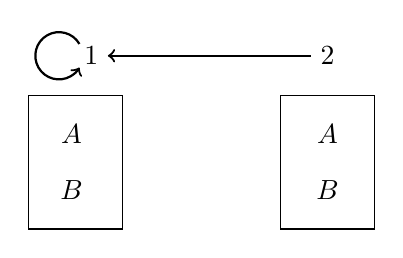
\begin{tikzpicture}
		\node (atom1) at (0,1) {1};
		\node (atom2) at (3,1) {2};
		\node (atom3) at (-0.25,0) {$A$};
		\node (atom4) at (3,0) {$\enot A$};
		\node (atom5) at (-0.25,-0.7) {$\enot B$};
		\node (atom6) at (3,-0.7) {$B$};
		\draw[->, thick] (atom1)+(-0.15,0.15) arc (-330:-30:.3);
		%\draw[->, thick] (atom2)+(0.15,-0.15) arc (-150:150:.3); 
		\draw[<-, thick] (atom1) -- (atom2);
		\draw (-0.8,-1.2) rectangle (0.4,0.5);
		\draw (2.4,-1.2) rectangle (3.6,0.5);
	\end{tikzpicture}
\end{center}
So lesen Sie die Interpretation aus diesem Diagramm ab: Sie enthält nur zwei Welten, 1 und 2. Die Pfeile zwischen den Welten repräsentieren die Zugänglichkeitsbeziehung. 1 und 2 greifen also beide auf 1 zu (beide erachten 1 als möglich), aber weder 1 noch 2 greifen auf 2 zu (beide erachten 2 als nicht möglich). Die Kästchen unter den Welten zeigen uns an, welche einfachen Sätze in diesen Welten wahr sind: $A$ ist wahr in 1, aber falsch in 2; $B$ ist falsch in 1, aber wahr in 2. In solche Kästchen kann man nur einen einfachen Satz oder seine Negation schreiben, nicht beide. Aus den Wahrheitswerten der einfachen Sätze in unseren Welten, können wir ersehen, welche Wahrheitswerte die komplexeren Sätze in jeder Welt erhalten. Bei dieser Interpretation sind zum Beispiel alle folgenden Sätze in $w_1$ wahr:
\begin{itemize}
	\item[]$A\eand\enot B$, $B\eif A$, $\ediamond A$, $\ebox\enot B$
\end{itemize}
Wenn Sie nicht diagrammatisch denken wollen, dann können Sie eine Interpretation auch wie folgt darstellen:
\begin{itemize}
	\item[$W$:]$1,2$
	\item[$R$:]$\langle 1,1\rangle, \langle 2,1\rangle$
	\item[]$\nu_{1}(A)=T, \nu_{2}(B)=F, \nu_{2}(A)=F, \nu_{2}(B)=T$
\end{itemize}
Sie werden in Kürze Gelegenheit haben, einige eigene Interpretationen zu erarbeiten, wenn wir uns mit \emph{Gegeninterpretationen} befassen.

\section{Eine Semantik für das System \mlK}
\label{SemanticsK}

Wir können nun alle semantischen Begriffe der WFL auf die ML ausdehnen:
\factoidbox{
	\begin{itemize}
		\item  $\metav{A}_1,\metav{A}_2, \dots \metav{A}_n\therefore\metav{C}$ ist \define{modal gültig} genau dann, wenn es in keiner Interpretation eine Welt gibt in der $\metav{A}_1,\metav{A}_2, \dots \metav{A}_n$ alle wahr sind und $\metav{C}$ falsch ist.
		
		\item $\metav{A}$ ist eine \define{modale Wahrheit} genau dann, wenn $\metav{A}$ in jeder Welt jeder Interpretation wahr ist.
		
		\item $\metav{A}$ ist ein \define{modaler Widerspruch} genau dann, wenn $\metav{A}$ in jeder Welt jeder Interpretation falsch ist.
		
		\item $\metav{A}$ ist \define{modal erfüllbar} genau dann, wenn $\metav{A}$ in zumindest einer von zumindest einer Interpretation wahr ist.
	\end{itemize}
}
(Von nun an lassen wir die Qualifikationen `modal', `modaler' usw.\@ weg.)

Wir können auch unsere Verwendung von $\entails$ ausweiten. Allerdings müssen wir wieder Subskripte hinzufügen, so wie wir es mit $\proves$ getan haben. Wenn wir also sagen wollen, dass $\metav{A}_1,\metav{A}_2, \dots \metav{A}_n\therefore\metav{C}$ (modal) gültig ist, dann schreiben wir: $\metav{A}_1,\metav{A}_2, \dots \metav{A}_n\entails_\mlK\metav{C}$. 

Lassen Sie uns ein besseres Gefühl für die Semantik für das System \mlK{} bekommen, indem wir einige Gegeninterpretationen durcharbeiten. Betrachten Sie die folgende (falsche) Behauptung:
\begin{itemize}
	\item[]
	\begin{itemize}
		\item[]$\enot A\entails_\mlK \enot \ediamond A$
	\end{itemize}
\end{itemize}
Um eine Gegeninterpretation zu dieser Behauptung vorzulegen, müssen wir uns eine Interpretation ausdenken, die $\enot A$ in irgendeiner Welt $w$ wahr und $\enot\ediamond A$ in derselben Welt $w$ falsch macht. Hier ist eine solche Interpretation, dargestellt mittels eines Diagramms:
\begin{center}
	\begin{tikzpicture}
		\node (atom1) at (0,1) {1};
		\node (atom2) at (3,1) {2};
		\node (atom3) at (-0.25,0) {$\enot A$};
		\node (atom4) at (3,0) {$A$};
		\draw[->, thick] (atom1) -- (atom2);
		\draw (-0.8,-0.6) rectangle (0.4,0.5);
		\draw (2.4,-0.6) rectangle (3.6,0.5);
	\end{tikzpicture}
\end{center}
Es ist leicht einzusehen, dass dies eine Gegeninterpretation zu unserer Behauptung ist. Erstens, $\enot A$ ist wahr in Welt $1$. Und zweitens ist $\enot\ediamond A$ falsch in $1$: $A$ ist wahr in $2$, und $2$ ist von $1$ aus zugänglich. Es gibt also eine Welt in dieser Interpretation, in der $\enot A$ wahr und $\enot\ediamond A$ falsch ist. Also ist es nicht der Fall, dass $\enot A\entails_\mlK\enot\ediamond A$.

Warum haben wir das Subskript \mlK{} gewählt? Nun, es stellt sich heraus, dass es eine wichtige Beziehung zwischen dem System \mlK{} und der Definition der Gültigkeit gibt, die wir gerade gegeben haben. Insbesondere gelten die folgenden beiden Ergebnisse:
\begin{itemize}
	\item Wenn $\metav{A}_1,\metav{A}_2, \dots \metav{A}_n\proves_\mlK\metav{C}$, dann $\metav{A}_1,\metav{A}_2, \dots \metav{A}_n\entails_\mlK\metav{C}$
	\item Wenn $\metav{A}_1,\metav{A}_2, \dots \metav{A}_n\entails_\mlK\metav{C}$, dann $\metav{A}_1,\metav{A}_2, \dots \metav{A}_n\proves_\mlK\metav{C}$
\end{itemize}
Das erste Ergebnis wird als \emph{Korrektheitsresultat} bezeichnet, da es uns sagt, dass die Herleitungsregeln des Systems \mlK{} gute, solide Regeln sind: Wenn Sie ein Argument rechtfertigen können, indem Sie einen Beweis innerhalb des Systems \mlK{} liefern, dann ist dieses Argument wirklich gültig. Das zweite Ergebnis ist als \emph{Vollständigkeitsresultat} bekannt, da es uns sagt, dass die Regeln des Systems \mlK{} ausreichend sind, um alle gültigen Argumente zu erfassen: wenn ein Argument gültig ist, dann ist es möglich, einen Beweis in \mlK{} anzubieten, der es rechtfertigt.

Es ist natürlich eine Sache, diese Resultate anzupreisen, aber eine ganz andere, sie zu beweisen. Wir werden hier jedoch nicht versuchen, sie zu beweisen. Aber die Idee, die hinter dem Nachweis der Korrektheit steht, wird vielleicht deutlicher machen, wie strenge Unterbeweise funktionieren. 

In einem strengen Unterbeweis dürfen wir keine Annahmen von au{\ss}erhalb des strengen Unterbeweises verwenden, mit Ausnahme dessen, was wir mit $\ebox$E in den strengen Unterbeweis `importieren'. Wenn wir mit $\ebox$E $\ebox \metav{A}$ angenommen oder bewiesen haben, können wir mit $\ebox$E $\metav{A}$ innerhalb eines strengen Unterbeweises verwenden. In \mlK{} ist das die einzige Möglichkeit, einen Satz in einen strengen Unterbeweis zu importieren. Alles, was innerhalb eines strengen Unterbeweises bewiesen werden kann, muss also aus dem Satz $\metav{A}$ folgen, wobei wir au{\ss}erhalb des strengen Unterbeweises eben $\ebox \metav{A}$ haben. Stellen wir uns vor, dass wir darüber nachdenken, was in einer möglichen Welt in irgendeiner Interpretation wahr ist. Wenn wir wissen, dass $\ebox\metav{A}$ in dieser möglichen Welt wahr ist, dann wissen wir, dass $\metav{A}$ in allen zugänglichen Welten wahr ist. Also ist alles, was innerhalb eines strengen Unterbeweises bewiesen wird, in allen zugänglichen möglichen Welten wahr. Deshalb ist $\ebox$I eine solide Regel.

\section{Eine Semantik für System \mlT}
\label{SemanticsT}

Gerade haben wir gesagt, dass das System \mlK{} korrekt und vollständig ist. Was bedeutet das für die anderen Modalsysteme, die wir untersucht haben, nämlich \mlT, \mlSfour{} und \mlSfive? Nun, sie sind alle \emph{inkorrekt}, relativ zu der Definition von Gültigkeit, die wir oben gegeben haben. Zum Beispiel erlauben uns all diese Systeme, $A$ aus $\ebox A$ abzuleiten, obwohl $\ebox A \nentails_\mlK A$.

Bedeutet das, dass diese Systeme eine Zeitverschwendung sind? Ganz und gar nicht! Diese Systeme sind nur inkorrekt \emph{relativ zu der Definition der Gültigkeit, die wir oben gegeben haben}. (Oder, um Symbole zu verwenden, sie sind inkorrekt relativ zu $\entails_\mlK$.) Wenn wir es also mit diesen stärkeren modalen Systemen zu tun haben, müssen wir unsere Definition der Gültigkeit anpassen, damit sie zu diesen Systemen passt. An dieser Stelle kommen uns die Zugänglichkeitsbeziehungen wirklich gelegen.

Als wir die Idee einer Zugänglichkeitsbeziehung einführten, sagten wir, dass es jede beliebige Beziehung zwischen Welten sein könnte, die Ihnen gefällt: Sie könnten jede Welt mit jeder Welt in Beziehung setzen, keine Welt mit irgendeiner Welt oder irgendetwas dazwischen. Dieses Bild der Zugänglichkeitsbeziehung war Hintergrund unserer Definition von $\entails_\mlK$. Aber wenn wir wollen, können wir die Zugänglichkeitsbeziehung etwas einschränken. Beispielsweise können wir darauf bestehen, dass sie \define{reflexiv} sein muss:
\begin{itemize}
	\item $\forall wRww$
\end{itemize}
Zu Deutsch: jede Welt ist sich selbst zugänglich. Oder: jede Welt erachtet sich selbst als möglich. Wenn wir diese Einschränkung annehmen, können wir eine neue Definition der Gültigkeit, $\entails_\mlT$, einführen:
\factoidbox{
	$\metav{A}_1,\metav{A}_2, \dots \metav{A}_n\entails_\mlT \metav{C}$ genau dann, wenn es in keiner Interpretation, die eine reflexive Zugänglichkeitsbeziehung hat, eine Welt gibt in der $\metav{A}_1,\metav{A}_2, \dots \metav{A}_n$ alle wahr sind und $\metav{C}$ falsch ist.
}
Wir haben das \mlT{} Subskript an $\entails$ angehängt, weil das System \mlT{} korrekt und vollständig relativ zu dieser neuen Definition der Gültigkeit ist:
\begin{itemize}
	\item Wenn $\metav{A}_1,\metav{A}_2, \dots \metav{A}_n\proves_\mlT\metav{C}$, dann $\metav{A}_1,\metav{A}_2, \dots \metav{A}_n\entails_\mlT\metav{C}$
	\item Wenn $\metav{A}_1,\metav{A}_2, \dots \metav{A}_n\entails_\mlT\metav{C}$, dann $\metav{A}_1,\metav{A}_2, \dots \metav{A}_n\proves_\mlT\metav{C}$
\end{itemize}
Wie vorher schon werden wir nicht versuchen, die Korrektheits- und Vollständigkeitsresultate zu beweisen. Es ist jedoch relativ leicht einzusehen, wie das Beharren darauf, dass die Zugänglichkeitsbeziehung reflexiv sein muss, die R\mlT{}-Regel rechtfertigen wird:
\factoidbox{
	\[\begin{nd}
		\have[m]{m}{\ebox \metav{A}}
		\have[\, ]{n}{\metav{A}}\rt{m}
	\end{nd}\]
}
Um dies einzusehen, stellen Sie sich einfach vor, Sie versuchen, eine Gegeninterpretation zu dieser Behauptung zu finden.
\[
\ebox \metav{A}\entails_\mlT \metav{A}
\]
Hierzu müssten wir eine Welt konstruieren, $w$, in der $\ebox \metav{A}$ wahr, aber $\metav{A}$ falsch ist. Wenn nun aber $\ebox \metav{A}$ in $w$ wahr ist, dann muss $\metav{A}$ in allen von $w$ aus zugänglichen Welten wahr sein. Aber da die Zugänglichkeitsbeziehung reflexiv ist, ist $w$ von $w$ aus zugänglich. Also muss $\metav{A}$ in $w$ wahr sein. Aber jetzt muss $\metav{A}$ in $w$ wahr \emph{und} falsch sein. Widerspruch!

\section{Eine Semantik für \mlSfour}
\label{SemanticsS4}

Wie sonst könnten wir an unserer Definition der Gültigkeit feilen? Nun, wir könnten auch festlegen, dass die Zugänglichkeitsbeziehung \define{transitiv} sein muss:
\begin{itemize}
	\item $\forall w_1\forall w_2\forall w_3 ((Rw_1w_2 \eand Rw_2w_3)\eif Rw_1w_3)$
\end{itemize}
Zu Deutsch: wenn $w_1$ Zugang zu $w_2$ hat, und $w_2$ Zugang zu $w_3$, dann hat $w_1$ Zugang zu $w_3$. Oder: wenn $w_1$ $w_2$ als möglich erachtet, und $w_2$ $w_3$ als möglich erachtet, dann erachtet $w_1$ auch $w_3$ als möglich. Wenn wir diese Einschränkung unserer Zugänglichkeitsbeziehung annehmen, dann können wir wieder eine neue Definition der Gültigkeit, $\entails_\mlSfour$, einführen:
\factoidbox{
	$\metav{A}_1,\metav{A}_2, \dots \metav{A}_n\entails_\mlSfour \metav{C}$ genau dann, wenn es in keiner Interpretation, die eine reflexive und transitive Zugänglichkeitsbeziehung hat, eine Welt gibt in der $\metav{A}_1,\metav{A}_2, \dots \metav{A}_n$ alle wahr sind und $\metav{C}$ falsch ist.
}
Wir haben das \mlSfour{} Subskript an $\entails$ angehängt, weil das System \mlSfour{} korrekt und vollständig relativ zu dieser neuen Definition der Gültigkeit ist:
\begin{itemize}
	\item Wenn $\metav{A}_1,\metav{A}_2, \dots \metav{A}_n\proves_\mlSfour\metav{C}$, dann $\metav{A}_1,\metav{A}_2, \dots \metav{A}_n\entails_\mlSfour\metav{C}$
	\item Wenn $\metav{A}_1,\metav{A}_2, \dots \metav{A}_n\entails_\mlSfour\metav{C}$, dann $\metav{A}_1,\metav{A}_2, \dots \metav{A}_n\proves_\mlSfour\metav{C}$
\end{itemize}
Wie vorher schon werden wir nicht versuchen, diese Resultate zu beweisen. Es ist jedoch relativ leicht zu erkennen, wie das Beharren darauf, dass die Zugänglichkeitsbeziehung transitiv sein muss, die \mlSfour-Regel rechtfertigt:
\factoidbox{
	\[\begin{nd}
		\have[m]{m}{\ebox\metav{A}}
		\open
		\hypo[\ ]{k}{\ebox}
		\have[\ ]{n}{\ebox\metav{A}}\rfour{m}
	\end{nd}\]
}
Die Idee, die den strengen Unterbeweisen zugrunde liegt, ist, dass Unterbeweise Wege sind, Dinge zu beweisen, die in allen zugänglichen Welten wahr sind. Die R$\mathbf{4}$-Regel bedeutet also, dass immer dann, wenn $\ebox \metav{A}$ wahr ist, $\ebox \metav{A}$ in jeder zugänglichen Welt wahr ist. Mit anderen Worten, es muss sein, dass $\ebox\metav{A} \entails_\mlSfour \ebox\ebox\metav{A}$ gilt.

Um dies einzusehen, stellen Sie sich vor, dass Sie versuchen, eine Gegeninterpretation zu dieser Behauptung zu finden:
\begin{itemize}
	\item[]$\ebox\metav{A} \entails_\mlSfour \ebox \ebox \metav{A}$
\end{itemize}
Hierzu müssten wir eine Welt konstruieren, $w_1$, in der $\ebox\metav{A}$ wahr, aber $\ebox \ebox \metav{A}$ falsch ist. Wenn nun $\ebox \ebox \metav{A}$ in $w_1$ falsch ist, dann muss $w_1$ eine Welt, $w_2$, zugänglich sein, in der $\ebox\metav{A}$ falsch ist. Gleicherma{\ss}en, wenn $\ebox \metav{A}$ in $w_2$ falsch ist, dann muss $w_2$ eine Welt, $w_3$, zugänglich sein, in der $\metav{A}$ falsch ist. Wir haben gerade gesagt, dass $w_1$ auf $w_2$ und $w_2$ auf $w_3$ Zugang haben. Da wir nun aber darauf bestehen, dass die Zugänglichkeitsbeziehung transitiv ist, muss $w_1$ auf $w_3$ Zugang haben. Und da $\ebox\metav{A}$ in $w_1$ wahr ist und $w_3$ von $w_1$ aus zugänglich ist, folgt daraus, dass $\metav{A}$ in $w_3$ wahr ist. Also ist $\metav{A}$ in $w_3$ wahr \emph{und} falsch. Widerspruch!

\section{Eine Semantik für \mlSfive}
\label{SemanticsS5}

Lassen Sie uns die Zugänglichkeitsbeziehung noch auf eine weitere Art einschränken. Nun beharren wir darauf, dass sie \define{symmetrisch} ist:
\begin{itemize}
	\item $\forall w_1\forall w_2(Rw_1w_2 \eif Rw_2w_1)$
\end{itemize}
Zu Deutsch: wenn $w_1$ Zugang zu $w_2$ hat, dann hat $w_2$ Zugang zu $w_1$. Oder: wenn $w_2$ von $w_1$ als möglich erachtet wird, dann wird $w_1$ von $w_2$ als möglich erachtet. Logiker*innen nennen eine Beziehung, die reflexiv, transitiv und symmetrisch ist, eine \define{Äquivalenzbeziehung}. Wir können nun eine neue Definition der Gültigkeit, $\entails_\mlSfive $, einführen:
\factoidbox{
	$\metav{A}_1,\metav{A}_2, \dots \metav{A}_n\entails_\mlSfive  \metav{C}$ genau dann, wenn es in keiner Interpretation, deren Zugänglichkeitsbeziehung eine Äquivalenzbeziehung ist, eine Welt gibt, in der $\metav{A}_1,\metav{A}_2, \dots \metav{A}_n$ alle wahr sind und $\metav{C}$ falsch ist.
}
Wir haben das \mlSfive{} Subskript an $\entails$ angehängt, weil das System \mlSfive{} relativ zu dieser neuen Definition der Gültigkeit komplett und vollständig ist:
\begin{itemize}
	\item Wenn $\metav{A}_1,\metav{A}_2, \dots \metav{A}_n\proves_\mlSfive \metav{C}$, dann $\metav{A}_1,\metav{A}_2, \dots \metav{A}_n\entails_\mlSfive \metav{C}$
	\item Wenn $\metav{A}_1,\metav{A}_2, \dots \metav{A}_n\entails_\mlSfive \metav{C}$, dann $\metav{A}_1,\metav{A}_2, \dots \metav{A}_n\proves_\mlSfive \metav{C}$
\end{itemize}
Wie vorher schon werden wir nicht versuchen, diese Resultate zu beweisen. Es ist jedoch relativ leicht zu erkennen, wie das Beharren darauf, dass die Zugänglichkeitsbeziehung eine Äquivalenzbeziehung sein muss, die R$\mathbf{5}$-Regel rechtfertigt:
\factoidbox{
	\[\begin{nd}
		\have[m]{m}{\enot\ebox \metav{A}}
		\open
		\hypo[\ ]{k}{\ebox}
		\have[\, ]{n}{\enot\ebox\metav{A}}\rfive{m}
	\end{nd}\]
}
Die Regel besagt, dass wenn $\metav{A}$ nicht notwendig ist, d.h.\@ in einer zugänglichen Welt falsch ist, dann ist es in keiner zugänglichen Welt notwendig. Wir haben also $\enot\ebox \metav{A} \proves_\mlSfive  \ebox\enot\ebox \metav{A}$.

Um dies einzusehen, stellen Sie sich vor, Sie versuchen eine Gegeninterpretation zu dieser Behauptung zu finden:
\[
\enot\ebox\metav{A} \entails_\mlSfive  \ebox \enot\ebox \metav{A}
\]
Hierzu müssten wir eine Welt konstruieren, $w_1$, in der $\enot\ebox\metav{A}$ wahr ist, aber $\ebox \enot\ebox \metav{A}$ falsch ist. Wenn nun $\enot\ebox\metav{A}$ in $w_1$ wahr ist, dann muss $w_1$ zu irgendeiner Welt, $w_2$, Zugang haben, in der $\metav{A}$ falsch ist. Gleicherma{\ss}en, wenn $\ebox \enot\ebox \metav{A}$ in $w_1$ falsch ist, dann muss $w_1$ zu einer Welt, $w_3$, Zugang haben, in der $\enot\ebox \metav{A}$ falsch ist. Da wir nun darauf bestehen, dass die Zugänglichkeitsbeziehung eine Äquivalenzbeziehung und somit \emph{symmetrisch} ist, können wir daraus schlie{\ss}en, dass $w_3$ zu $w_1$ Zugang hat. Somit hat $w_3$ zu $w_1$ und $w_1$ zu $w_2$ Zugang. Da wir nun wiederum darauf bestehen, dass die Zugänglichkeitsbeziehung eine Äquivalenzbeziehung und damit \emph{transitiv} ist, können wir daraus herleiten, dass $w_3$ auf $w_2$ zugreift. Aber vorhin sagten wir, dass $\enot\ebox \metav{A}$ in $w_3$ falsch ist, was impliziert, dass $\metav{A}$ in jeder Welt wahr ist, zu der $w_3$ Zugang hat. Also ist $\metav{A}$ wahr \emph{und} falsch in $w_2$. Widerspruch!

In der Definition von $\entails_\mlSfive $ haben wir festgelegt, dass die Zugänglichkeitsbeziehung eine Äquivalenzbeziehung ist. Aber es gibt noch eine andere Möglichkeit, einen Gültigkeitsbegriff, der zu \mlSfive{} passt, zu kriegen. Anstatt festzulegen, dass die Zugänglichkeitsbeziehung eine Äquivalenzbeziehung ist, könnten wir festlegen, dass es sich um eine \define{universelle} Beziehung handelt:
\begin{itemize}
	\item $\forall w_1\forall w_2Rw_1w_2$
\end{itemize}
Zu Deutsch: jede Welt hat zu jeder Welt Zugang. Oder: jede Welt erachtet jede Welt als möglich. Mit dieser Beschränkung der Zugänglichkeitesbeziehung hätten wir $\entails_\mlSfive $ wie folgt definieren können:
\factoidbox{
	$\metav{A}_1,\metav{A}_2, \dots \metav{A}_n\entails_\mlSfive  \metav{C}$ genau dann, wenn es in keiner Interpretation, die eine universelle Zugänglichkeitsbeziehung hat, eine Welt gibt, in der $\metav{A}_1,\metav{A}_2, \dots \metav{A}_n$ alle wahr sind und $\metav{C}$ falsch ist.
}
Wenn wir $\entails_\mlSfive$ so definieren würden, würden wir für \mlSfive{} immer noch die gleichen Korrektheits- und Vollständigkeitsresultate erhalten. Was sagt uns das? Nun, es bedeutet, dass wir, wenn wir eine Art von Notwendigkeit untersuchen, laut der \emph{jede} Welt relativ zu \emph{jeder} Welt möglich ist, \mlSfive{} verwenden sollten. Darüber hinaus gehen die meisten Philosoph*innen davon aus, dass die Begriffe der Notwendigkeit, um die es ihnen am meisten geht, wie die \emph{logische} Notwendigkeit und die \emph{metaphysische} Notwendigkeit, genau von dieser Art sind. So ist \mlSfive{} das modale System, das die meisten Philosoph*innen die meiste Zeit nutzen.

\practiceproblems

\problempart
Legen Sie Gegeninterpretationen zu den folgenden falschen Behauptungen vor:
\begin{earg}
	\item $\enot P \entails_\mlK \enot\ediamond P$
	\item $\ebox(P \eor Q)\entails_\mlK \ebox P \eor \ebox Q$
	\item $\entails_\mlK \enot \ebox (A\eand \enot A)$
	\item $\ebox A\entails_\mlK A$
\end{earg}

\problempart
Legen Sie Gegeninterpretationen zu den folgenden falschen Behauptungen vor:
\begin{earg}
	\item $\ediamond A\entails_\mlSfour \ebox\ediamond A$
	\item $\ediamond A, \ebox (\ediamond A \eif B)\entails_\mlSfour\ebox B$
\end{earg}

\problempart
Legen Sie Gegeninterpretationen zu den folgenden falschen Behauptungen vor:
\begin{earg}
	\item $\ebox (M\eif O),\ediamond M\entails_\mlT O$
	\item $\ebox A\entails_\mlT \ebox \ebox A$
\end{earg}

\section*{Weitere Lektüre}

Die modale Logik ist ein sehr gro{\ss}er Teilbereich der Logik. Wir haben nur an der Oberfläche gekratzt. Wenn Sie mehr über die modale Logik erfahren möchten, finden Sie hier einige Lehrbücher, die Sie konsultieren können.
\begin{itemize}
	\item Hughes, G. E., \& Cresswell, M. J. (1996). \emph{A New Introduction to Modal Logic}, Oxford: Routledge.
	\item Priest, G. (2008). \emph{An Introduction to Non-Classical Logic}, 2nd ed., Cambridge: Cambridge University Press.
	\item Garson, J. W. (2013). \emph{Modal Logic for Philosophers}, 2nd ed., Cambridge: Cambridge University Press.
\end{itemize}

Keiner dieser Autoren formuliert seine modalen Beweissysteme so, wie wir es getan haben, aber die ähnlichste Formulierung gibt Garson.